

\documentclass[12pt]{article}
\usepackage[utf8]{inputenc}
\usepackage{graphicx}
\usepackage{url}
\usepackage{xcolor}
\usepackage{comment}
\usepackage{mathptmx} % Times New Roman font
\usepackage{geometry} % margins
\usepackage{authblk} % affiliations
\usepackage{indentfirst} % indent first paragraph
\usepackage{amsmath}
\usepackage{amsfonts}
\usepackage{amssymb}
\usepackage{caption}
\captionsetup[table]{position=bottom}   %% or below
\usepackage{hyperref}
%next two packages allows table to float within text
\usepackage{float}
\restylefloat{table}
\usepackage{enumitem} %to make lists
\setlist[description]{leftmargin=\parindent,labelindent=\parindent}







%%%%%%%%%%%%%%%%%%%%%%%%%%%%%%%%%%%%%%%%%%%
% Page Setup
\pagenumbering{gobble}
\geometry{margin=1in}

% separation between title/authors/affiliations
\setlength{\affilsep}{1.5em}
% make paragraph indent larger
\setlength{\parindent}{3.5em}

%Sets the size of the affiliations to that of footnotes
\renewcommand\Affilfont{\footnotesize}

\makeatletter
 \def\@maketitle{%
   \newpage
   \begin{center}%
   \let \footnote \thanks
     {\huge\bfseries \@title \par}%
     \vskip \@affilsep%
     {\large%
         \begin{tabular}[t]{c}%
         \@author\\
         contact: \href{mailto:\contact}{\contact}
       \end{tabular}\par}%
   \end{center}}
 \makeatother
%end Page Setup
%%%%%%%%%%%%%%%%%%%%%%%%%%%%%%%%%%%%%%%%%%%
%Title & Affiliation Settings
\title{Is Conversation Zipfian?}
\def\contact{jkilfoyle@zagmail.gonzaga.edu}
\author[1]{{Jeb Kilfoyle}}
\author[1]{Paul De Palma}
\author[1]{Phillip Fishburn}
\author[1]{Alex Giacobbi}
\author[1]{Allison Hayes}
\author[2]{Joseph Stover}
\author[3]{Mark VanDam}
\affil[1]{Department of Computer Science, Gonzaga University}
\affil[2]{Department of Mathematics, Gonzaga University}
\affil[3]{Department of Speech and Hearing Sciences, Washington State University}
%%%%%%%%%%%%%%%%%%%%%%%%%%%%%%%%%%%%%%%%%%%

\begin{document}
\maketitle  %Generate title and the affiliations
\section*{\centering\large Abstract}
\noindent Zipf's law describes the relationship between the frequency of words in a large corpus and their rank.  Its most basic form is a harmonic series, indicating that the frequency of words is inversely proportional to their rank.  The past two decades have seen the emergence of usage-based and cognitive approaches to language study.  A key observation of these approaches is that speech differs in substantial and structural ways from writing.  Except for a few older analyses performed on very small corpora, all studies of Zipf's law have been done on written corpora.  The primary research question is this: "Do the words which comprise transcribed speech corpora follow a Zipfian distribution?"  This paper examines several transcribed speech corpora to see if spoken words form a Zipfian distribution.  In addition, many presentations Zipf's law, use relatively informal methods to determine whether given distribution is Zipfian.  A log-log plot of frequency against rank with slope of -1 is frequently enough for the distribution to be judged Zipfian.  This paper uses the Kolgomorov Smirnov statistic in conjunction with more rigorous and recently developed statistical techniques to judge whether a corpus under examination is Zipfian. Some previous "Zipfian" are shown to be non-Zipfian.  Speech, in most cases, is shown to be Zipfian. \\

\noindent Acknowledgements: The authors would like to thank Robert and Clare McDonald and the McDonald Work-Award Program for their generous and continuous support.


\section{Introduction}

The title of this article is posed as a question, but implies answers to two preceding questions, each with an embedded prior question: 1) What is what is meant by "conversation," (and why do we care about it); and 2) What is meant by "Zipfian" (and how do we know it when we see it).  Since we have framed question 1 by its modifier in question 2, we begin with Zipfianness. Any student of linguistics can confidently recite Zipf's Law.  The frequency of a word in a language is inversely proportional to its rank.  More precisely, the second ranked word is half as frequent as the first, the third is one-third as frequent as the first, and so on:
\begin{center}
\[\frac{1}{2}, \frac{1}{3}, \frac{1}{4},...\]
\end{center}

It is a remarkable result, usually attributed to George Kingsley Zipf, a Harvard philologist  whose 1949 book, \emph {Human Behavior and the Principle of Least Effort} (Zipf, 1949), manages to sound contemporary and quaint at the same time: "Nearly twenty-five years ago, it occurred to me that we might gain considerable insight into the mainsprings of human behavior if we viewed it purely as a natural phenomenon like everything else in the universe, and if we studied it with the same dispassionate objectivity with which one is wont to study, say, the social behavior of bees, or the nestbuilding habits of birds" (Zipf, 1949, p. v).\footnote[1]{Though Newman (2005) says pride of first place actually belongs to the German physicist, Felix Auerbach, who observed in 1913 that city populations form what we now call a Zipfian distribution.  Auerbach's interests ranged widely. In 1925 he published a book with the distinctively modern-sounding title,\emph{ The Fear of Mathematics and Conquering It (Die Furcht vor der Mathematik und ihre Überwindung).} Zipf first presented his ideas in a 1932 monograph (Zipf, 1932).  It is not surprising that in a world without Google Scholar he does not cite Auerbach's German paper, though he himself was an "Instructor in German," according to the frontispiece of his 1932 article. This seems yet another instance of co-discovery.}  Relying on a previously published and hand-counted indices of words and their frequencies in James Joyce's \emph{Ulysses}, and a sample of American newspapers, he produced the familiar log-log plot for word frequency against rank along the idealized line with slope = -1 that is found in modern papers on Zipf's law.  See, for example Ha, \emph{et al. (2002)}. \\
\indent As it happens, word frequencies are not the only natural phenomenon that follow Zipf's Law. Magnitudes of earthquakes, intensity of solar flares, citations of scientific paper, web hits, wealth, family names, and (with a nod to Aurebach) city populations all appear to follow a Zipfian distribution (Newman, 2005).  What these phenomenon have in common is intuitively obvious.  There are very few of each with high numbers (rich people, large earthquakes, heavily cited papers, etc.), and a great many with low numbers (poor people, small earthquakes, uncited papers, etc.).   Figure 1 is a plot of the cumulative distribution of wealth among the world's five hundred richest people (as of 3/8/2019) against their rank.  Figure 2 shows a log-log plot of the same data. The plots tell us that although all five hundred of the world's richest people may be rich, a very few are the richest of all (\emph{arrepim}, 2020; \emph{Bloomberg Billionaire's Index}, 2020).  The plots can seem mysterious.  Why, exactly, does the log-log plot of cumulative wealth against wealth rank form a straight line of slope approximately -1? And, for that matter, what closed form formula produces the plot in Figure 1?  Mathematical treatments of Zipf's Law tend to be either forbiddingly formal or so simple as to miss its richness.  See, for example Baayen (2001).   The next section, a clear, yet complete discussion of Zipf's Law, is intended fill a whole in word distribution studies.  

\section{From Zipf's Law to Power Laws}

\indent 
Perhaps the easiest way to begin a discussion of Zipf's Law is to begin with Zipf himself.  Early on in his 1947 book, he presents a formula derived from observing word frequencies in James Joyce's \emph{Ulysses} \footnote[2]{Zipf used the Hanley Index to the book (Hanley, 1937). We have downloaded and tokenized the text available from Project Gutenberg (https://www.gutenberg.org). The numbers in table 1 differ slightly from Zipf's, due most likely to differences in editions and tokenization techniques.  The inferences licensed by the numbers are identical to Zipf's, however.}.  Let \emph{f} be the frequency of occurrence of a word occurs in a text, and \emph{r} the rank of that word.  Then their product is a constant:

\setlength{\abovedisplayskip}{1pt}
\setlength{\belowdisplayskip}{1pt}
\begin{center}
\begin{equation*}
\begin{aligned}
r\, x\, f\, =\, C\hspace{4em (1)}
\end{aligned}
\end{equation*}
\end{center}

Table 1 is our version of Zipf's table of selected ranks and frequencies.  The ranks shown were chosen by Zipf, though his lowest rank was 29,899 reflecting more word types generated by Hanley's (see footnote 2) tokenization algorithm.  

\begin{table}[H]
\begin{center}
 \begin{tabular}{||l l l|| }
 \hline
 Rank ($r$) &  Freq ($f)$ & $C$ \\
 \hline
    10 & 2561& 25610    \\
    20 & 1301 & 26020   \\
    30 & 947 & 28410    \\
    40 & 720 & 28800    \\
    50 & 565 & 28250    \\
    100 & 274 & 27400   \\
    500 & 52 & 26000    \\
    1000 & 26 & 26000   \\
    2000 & 13 & 26000   \\
    3000 & 8 & 24000    \\
    4000 & 6 & 24000    \\
    5000 & 5 & 25000    \\
    10000 & 2 & 20000   \\
    20000 & 1 & 20000   \\
    29121 & 1 & 29121   \\
  \hline
\end{tabular} 
\caption{A Sample of Ranks with Frequencies in James Joyce's \emph{Ulysses}}
\end{center}
\end{table}
Zipf himself made much of the third column, "which is approximately the same for all the different ranks" (Zipf, 1947, p. 23), though he never defines "approximately."  If we omit words which appear only once in the text, the standard deviation of column three is 2,407.   If we omit the 10 most frequently occurring words as well, the standard deviation drops to 936.  "Approximately" seems appropriate in either case. 

The computation of rank times frequency led Zipf to another observation that is not often mentioned in the literature on Zipfian distributions.  This is $r X f$ times a text-specific constant yields an approximation of the size of the text itself.   The constant in the case of \emph{Ulysses} is 10.  If we multiply the values in the third column, omitting the word groups as noted above, the approximations are 236,364 and 260,583, respectively.   The number of tokens in the Project Gutenberg edition of \emph{Ulysses} is 263,392, a reasonable approximation.   We next take a quick look at how this follows from Zipf's first observation, namely that rank times frequency generates an approximate constant for the text under discussion.

Since $r X f = C$, and, of course, $f = \frac{C}{r}$, then, with $N$ the number of words in the text and $C$ the proportionality constant, word frequencies decrease in proportion to a simple harmonic series:

\setlength{\abovedisplayskip}{1pt}
\setlength{\belowdisplayskip}{1pt}
\begin{center}
\begin{equation*}
\begin{aligned}
1,\frac{1}{2},\frac{1}{3},\frac{1}{4},...\frac{1}{\emph{N}}\hspace{4em (3)}
\end{aligned}
\end{equation*}
\end{center}
\noindent
With a few adjustments, (3) can be reformulated as a probability sequence, and from that, the use of Zipf's law to approximate the number of words in a text emerges. Suppose for a given text, $w_r$ is the word of rank $r$, $f_r$ is the frequency of $w_r$, and $p_r$ is the probability of word $w_r$ occurring the text, then,
\begin{center}
$p_r\, =\, \frac{f_r}{N}$    \hspace{4em (4)}
\end{center}
\noindent
















\section{Materials and Methods}
\subsection{Goodness of Fit Test}

This study compared word frequencies from seven corpora of transcribed spoken language with the Brown Corpus of written language.  Table 1 provides a list of the corpora by type. 

\begin{table}[H]
\caption{Table 1: Speech Corpora Analyzed}
\begin{center}
\begin{tabular}{ |l|l|l|l| } 
 \hline
 Buckeye & Spoken & 10 & Pitt, 2007 \\ 
 MiCase & Spoken & 10 & Simpson, 2002 \\
 Fisher & Spoken & 10 & Cieri et \emph(al), 2004 \\ 
 ATIS   & Spoken & 10 & Dahl, 1995 \\
 Santa Barbara & Spoken & 10 & Du bois, 2000-2005 \\
 Czech Telephone & Spoken & 10 & Korvas et \emph(al), 2014 \\
 Brown & Written & 10 & Francis and Kucera, 1964 \\
 \hline
\end{tabular}
\end{center}
\end{table}

Following Le et \emph{al} (2002), we generated unigram, bigram, and trigram frequency lists for each of these corpora, as well as a frequency list over all gram sizes.  These frequency lists were then examined to see whether they were consistent with Zipf’s as defined in (1),
\setlength{\abovedisplayskip}{1pt}
\setlength{\belowdisplayskip}{1pt}
\begin{center}
\begin{equation*}
\begin{aligned}
p(x) &= Cx^{-\alpha}\hspace{4em (2)}
\end{aligned}
\end{equation*}
\end{center}
where C is a proportionality constant to be explained below, x is the rank of the word, and alpha is the exponential scaling parameter used in fitting experimental data to an ideal power law.  So, for example, if $\alpha=1$, $p(1) = C$, $p(2)=\frac{c}{2}$, and $p(3)=\frac{c}{3}$.... Each p(x) is the probability that the $x^{th}$ most frequent word or word sequence would be selected from random sample.
\\ We used the methodology suggested in Clauset \emph{et al.} (2009) to determine whether the observed word (or word sequence)\footnote[2]{from now on, we will refer to words and word sequences as \emph{grams}} is best fit by a theoretical power law. What follows is a recap of their methodology.

Power-law behavior usually breaks down in the tail of the distribution, because the low number of expected occurrences are swamped by noise and non-distribution related effects. Therefore, it is important to establish a reasonable lower bound, $x_{min}$  for power law behavior.  The technique is sensitive to the choice of $x_{min}$.  Set it too high and legitimate data is discarded.  Set it too low and we allow non-power-law data into our distribution. Clauset's approach for estimating $x_{min}$ is to choose the value which minimizes the Kolmogorov-Smirnov (KS) statistic. The KS statistic is a measure of the maximum distance between the cumulative density functions (CDF)of the data (Sn(x) in Figure 1) and the theoretical model (Fx(x) in Figure 1). Note that the graph illustrates the KS statistic over an arbitrarily chosen data set (Springer, 2020).

\begin{figure}[h!]
\centering
  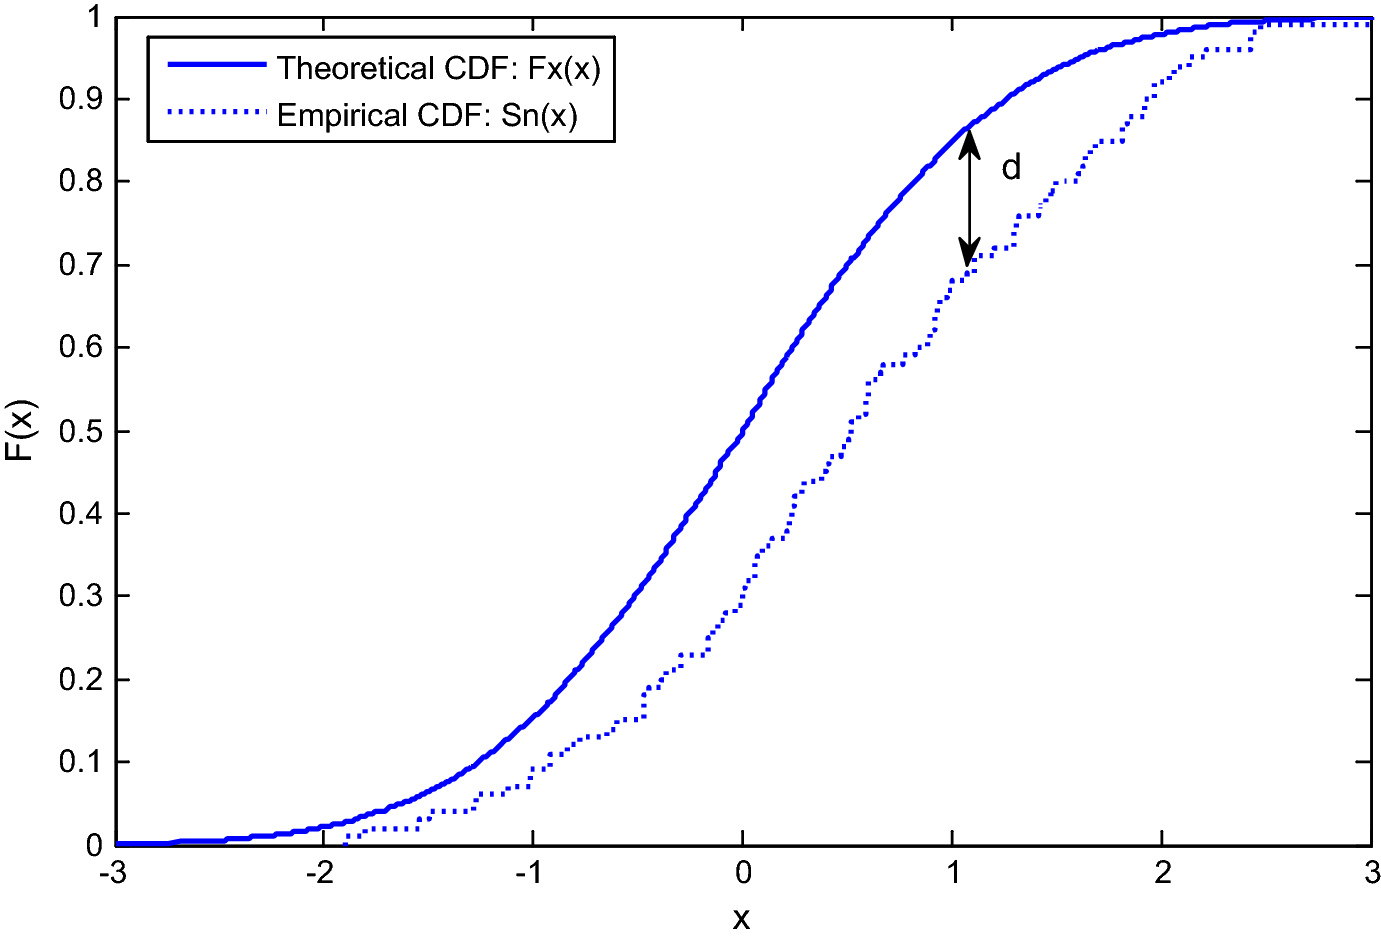
\includegraphics[scale=.75]{ks_test.png}\\
  \caption{Figure 1: KS Distance}
\end{figure}

\begin{center}
\setlength{\abovedisplayskip}{1pt}
\setlength{\belowdisplayskip}{1pt}
\end{center}  

In (2), Sn(x) is the distribution of the corpus under consideration, the CDF, and Fx(X), the power law distribution from (1), is the theoretical model.
\begin{equation*}
\begin{aligned}
d &= max|F(x)-P(x)|\ x\geq x_{min}\hspace{4em (2)}
\end{aligned}
\end{equation*} 

Having established a lower bound for our power-law behavior, we can now calculate a scaling parameter $\alpha$, which turns out to be a  maximum likelihood estimation (MLE) which is given by the formula:

\begin{equation*}
\begin{aligned}
\alpha = 1 +\left[ \sum_{i=1}^{n}ln\frac{x_i}{x_{min}}\right]^{-1}\hspace{4em (3)}
\end{aligned}
\end{equation*} 

With these parameters, we can now perform a goodness of fit test for our best fit model, in this case the power law for which we have calculated an $\alpha$ in equation (10). In this case, the best fit model is how well a given frequency distribution fits a power law distribution. We calculate the KS statistic between our empirical data and our best fit model.  We then create many synthetic data sets by sampling a discrete power-law distribution equivalent to our best fit. Synthetic data sets (SDS) are computationally generated artifacts for use in the best fit process.  They enable the calculation of p-values.  An SDS is generated by uniformly sampling a continuous interval, [0,1]  and transforming the results so that they lie on a discrete power law distribution (Clauset, Shalizi, and Newman, 2009, Appendix D).  We then fit each synthetic data set to its own power-law model, by calculating its KS statistic relative to its best fit model. Figure 1 illustrates this process.  

In this study, a p-value is the number of datasets with a KS greater than its best fit model divided by the number of synthetic data sets.   For example, one would expect the Brown corpus of written text, the first million word corpus of English (Jurafsky and Martin, 2009), to be Zipfian.  In fact, we find that it has a p-value of 0.37.  Clauset \emph{et al} (2009) empirically determined that a p-value $\geq$ .1 is significant evidence that the data is drawn from a power law distribution.We can now state our hypothesis with precision:

\begin{itemize}
\item $H^0$: The data is drawn from a power-law distribution
\item $H^1$: The data is not drawn from a power-law distribution
\end{itemize}

The number of synthetic datasets needed, of course, will affect the accuracy of the p-value, where the accuracy is expressed as the p-value plus or minus some $\epsilon$. The empirical relation between N, the number of synthetic datasets and  $\epsilon$ is given in: 

\begin{equation*}
\begin{aligned}
N = \frac{1}{4{\epsilon}^2}\hspace{4em (4)}
\end{aligned}
\end{equation*}

For our work we set N to 5000 data sets, giving us $$\epsilon  = 7.07*10^{-3}$$ This guarantees a p-value with an uncertainty less than  $\pm0.01$. We use the more conservative $p \geq 0.10$ as a cutoff for power-law behavior. p-values less than 0.10 are unlikely to demonstrate power-law behavior. At this point in the analysis, we could compare our proposed power law distribution with other possible distributions, but this would be pointless since our p-value rules out a power law distribution.  If, however, the p-value is significant, we should still compare it to other distributions which might fit it better. 

Note that we could introduce more parameters to provide a better fit, but to do so might be to overfit the distribution.  Said another way, we might fit our data with a complex polynomial but this would not necessarily give us insight into the distribution.  On the other hand other distributions such as exponential, poisson and lognormal occur frequently in nature and bear a closer look.

This would rule out distributions that might reasonably give rise to heavy tailed natural phenomena, such as exponential, poisson and lognormal distributions. (Note to self: Be sure to Find citation of these distributions occurring in nature and insert them here.) To compare power-law distributions to other distributions, we used a likelihood ratio test as proposed by Clauset, Shalizi, and Newman (2009,as cited in Vuong, 1989).

\subsection{Likelihood Ratio Test}

To determine which of two hypothetical distributions is more likely,  we  calculate the product of the probabilities of each of data point for each data set and choose the highest number.  The individual probabilities come from the probability density function itself, Equation (1), for example.  The result, since it is a product of many small decimal fractions is likely to be very small. To make the result more apparent, we take its logarithm. 

In addition to the likelihood ratio, we also derive a p-value to indicate the significance of the ratio test.  A small p-value indicates a significant result.
Given probability density functions $p_{1}(x)$ and $p_{2}(x)$,  let $L_1$ be the likelihood of $p_1$ and $L_2$ be the likelihood of $p_2$ such that:

\begin{minipage}{0.25\linewidth}
\begin{equation*}
L_{1} = \prod_{i=1}^{n} p_{1}(x_{i})
\end{equation*}
\end{minipage}
\hspace{0.5cm}
and
\hspace{0.5cm}
\begin{minipage}{0.25\linewidth}
\begin{equation*}
L_{2} = \prod_{i=1}^{n} p_{2}(x_{i})
\end{equation*}
\end{minipage}

So the ratio R:
\begin{equation*}
R = \frac{L_{1}}{L_{2}} = \prod_{i=1}^{n}\frac{p_{1}(x_i)}{p_{2}(x_i)}
\end{equation*}

Taking the log, we get the log-likelihood ratio:
\begin{equation*}
\widetilde{R} = \sum_{i=1}^{n}\left[\ln p_{1}(x_i)-\ln p_{2}(x_i)\right]
\end{equation*}

Since each sample $x_{i}$ is independent of other samples, then by the central limit theorem, the difference of our log-likelihoods will tend toward a normal distribution for large values of n.

From this, we can derive a p-value for the probability that the log-likelihood ratio would be as large or larger than our observed value. Given the normal distribution between the log-likelihoods, we can calculate the p-value using the complementary error function (\emph{erfc}) of the resultant normal distribution, 

\begin{equation*}
p = |\textrm{\emph{erfc}}(\frac{\widetilde{R}}{\sqrt{2n\sigma}})|
\end{equation*}

It is worth noting that unlike the p-value associated with our goodness of fit test for the power-law, a small p-value, p $\leq$0.10 would imply a statistically insignificant result. Thus, our likelihood test can tell us which distribution is favored, how strongly it is favored, and whether the difference is significant.

\section{Results}

We begin with the goodness-of-fit test. Initially, we can observe that under a conservative p-value of p $\geq$ 0.10 shows that unigrams, i.e., words, in most of the corpora under examination are consistent with a Zipfian distribution. The exceptions were the Buckeye and ATIS corpora. If we used the more liberal cutoff of p $\leq$ 0.05 then only the ATIS corpus is disqualified.

The bigram case seems to be strongly non-Zipfian, with only the Czech bigrams giving evidence for power-law behavior. The trigrams are a mixed group, with the Buckeye, Santa Barbara and ATIS corpora qualifying. The quadgrams, like the bigrams, seem safely non-Zipfian, with only one corpus giving indication of power-law behavior. The combined n-grams case is mixed.  Given the strength of the results for unigrams and the mixed results for multiword sequences, the initial results cast doubt on the possibility of multi-word sequences being Zipfian. See Table 2.


\begin{table}[H]
\caption{Table 2: p-values by corpus}
\begin{center}
\begin{tabular}{ |l|l|l|l|l|l| } 
\hline
 Corpus & Unigram & Bigram & Trigram & Quadgram & All Gram\\ [0.5ex] 
 \hline
 Buckeye & 0.06 & 0.00 & 0.35 & 0.00 & 0.00 \\ 
 MiCase & 0.15 & 0.00 & 0.00 & 0.02 & 0.07\\
 Fisher & 0.78 & 0.00 & 0.00 & 0.03 & 0.00 \\ 
 ATIS & 0.00 & 0.00 & 0.31 & 0.35 & 0.00 \\
 Santa Barbara & 0.58 & 0.00 & 0.62 & 0.00 & 0.45 \\
 Czech Telephone & 0.15 & 0.76 & 0.00 & 0.00 & 0.47 \\
 \hline
\end{tabular}
\end{center}
\end{table}

The frequency counts of these distributions from peak ($x_{max}$) to cutoff ($x_{min}$) are shown in Table 3. As is apparent, in each corpus, the great bulk of the distribution lies within the peak and cutoff, and is being considered in the power law fit computation.

\begin{table}[H]
\caption{Table 3: $x_{min}$ and $x_{max}$ by corpus}
\begin{center}
\begin{tabular}{| *{11}{l|} }
    \hline
$x_{max}$, $x_{min}$    & \multicolumn{2}{l|}{Unigram}
            & \multicolumn{2}{l|}{Bigram}
                    & \multicolumn{2}{l|}{Trigram}
                            & \multicolumn{2}{l|}{Quadgram} 
                            & \multicolumn{2}{l|}{All Gram}\\
    \hline
Buckeye   &   11962  &   5  & 1383 & 2&   559  &   3  &   94  &   1  &   11962  &   5  \\
    \hline
MiCase   &   74644  &   38  &   7404  &   4  &   1451  &   4  &   250  &   4 & 74644 & 11  \\
    \hline
Fisher   &  322401 & 151 & 101464 & 3 & 17536 & 3 & 3393 & 5 & 322401 & 16\\
    \hline
ATIS   &  8098     &    1   &   2127    &   1    &      1348 &  7     &     500  &      4 & 8098 & 3 \\
    \hline
Santa Barbara   &  8075     &   7    &  1456     &      3 & 314& 3&  46      & 1      & 8075      &      9 \\    \hline
Czech Telephone   &   6732    &     8  &    1216   &    5   &  776     &     1  & 446       & 1     & 6732 & 16  \\
    \hline
\end{tabular}
\end{center}
\end{table}

Having looked at the goodness-of-fit test, we now compare the fit to the other distributions using the likelihood ratio test. Recall that for every log-likelihood ratio test there is a corresponding p-value.  Table 4 shows the comparison of the power law distribution to other distributions.  A p-value $\geq$ 0.10 indicates a significant comparison.  A positive ratio (R) favors the power law.  A negative ratio favors the alternative.  As can be seen, neither the Poisson nor the Exponential distributions significantly compare.  The log-normal distribution is muddier, with MiCase favoring power law, Santa Barbara and Czech Telephone favoring log-normal, with the others showing insignificant p-values.

\begin{table}[H]
\caption{Table 4: Comparison Test by corpus}
\begin{center}

\begin{tabular}{| *{7}{l|} }
    \hline
p, R& \multicolumn{2}{l|}{Log-normal}
            & \multicolumn{2}{l|}{Poisson}
                    & \multicolumn{2}{l|}{Exponential}\\
    \hline
Buckeye  & 0.06 & -1.82 & 0.00 & 6.85 & 0.00 & 7.80 \\
    \hline
MiCase & 0.50 & 0.67 & 0.00 & 6.48 & 0.00 & 7.11  \\
    \hline
Fisher   & 0.06 & -1.88 & 0.00 & 6.66 & 0.00 & 7.48\\
    \hline
ATIS   & 0.00 & -5.62 & 0.00 & 7.03 & 0.00 & 8.11\\
    \hline
Santa Barbara  & 0.43 & -0.79 & 0.00 & 6.91 & 0.00 & 13.67  \\
    \hline
Czech Telephone & 0.36 & -0.91 & 0.00 & 5.06 & 0.00 & 9.14   \\
    \hline
\end{tabular}
\end{center}
\end{table}

\section{Discussion}

In this study we have examined six corpora of spoken language.  From each corpus we developed collections of unigrams, bigrams, trigrams, quadgrams, along with a collection composed of the union of uni, bi, tri, and quadgrams. For each collection within each corpora we performed Clauset's test for goodness of fit.  Looking at our results for this test (Table 2), we find that four out of our six corpora were strongly Zipfian using a stringent cutoff ($p \geq 0.10$), and five out of six were consistent with a more relaxed cutoff ($p \geq 0.05$).

Ha, \emph{et al.} (2002) examined two written corpora, one in English. one in Chinese, using ngrams, bigrams, trigrams, and quadgrams.  Not surprisingly, the unigram colleciton was Zipfian.  Their paper also claimed to demonstrate that N-grams (2-5) and combined grams were also Zipfian.  They appear to have used linear regression to determine goodness of fit.  The log-log plots provided in the paper appear to give visual confirmation that the corpora follow a Zipfian distribution. 
(Note to Self: Insert log log plot ofg ATIS unigram, because it is by our test, non-zipfian, but will appear zipfian on log log plot)





\begin{thebibliography}{9}

\bibitem{arrepim}
\emph{arrepim: information, pure and simple} (2020, May 7).\\ 
\url{https://stats.areppim.com/listes/list_billionairesx19xwor.htm.}


\bibitem{Bloomberg}
\emph{Bloomberg Billionaire's Index} (2020, May 7). \\
\url{https://www.bloomberg.com/billionaires.}

\bibitem{Baayen}
Baayen, R. Harald (2001).  \emph{Word Frequency Distributions}. Dordrecht: Kluwer Academic Publishers.

\bibitem{Fisher}
Cieri, C., Miller, D., Walker, K. (2004, May). \emph{The Fisher Corpus: a Resource for the Next Generations of Speech-to-Text}. In LREC (Vol. 4) pp. 69-71. (note to self: fix this reference)

\bibitem{Clauset}
Clauset, A., Shalizi, C. R., Newman, M. E. J. (2009). Power-Law Distributions in Empirical Data. SIAM Review, 51(4), 661–703. doi:10.1137/070710111.


\bibitem{ATIS}
Dahl, Deborah A., et al. ATIS3 Test Data LDC95S26. (1995). Philadelphia: Linguistic Data Consortium.

\bibitem{SantaBarbara}
Du Bois, John W., Wallace L. Chafe, Charles Meyer, Sandra A. Thompson, Robert Englebretson, and Nii Martey. 2000-2005. Santa Barbara corpus of spoken American English, Parts 1-4. Philadelphia: Linguistic Data Consortium.

\bibitem{Brown}
Francis, W. N., Kucera, H. (1979). Brown Corpus manual: Manual of information to accompany a standard corpus of present-day edited American English for use with digital computers. Brown University, Providence, Rhode Island, USA.

\bibitem{Hanley}
Hanley, M.L. (1937). \emph{Word Index to James Joyce's Ulysses. Madison: University of Wisconsin Press}

\bibitem{CzechTelephone}
Korvas, M., Plátek, O., Dušek, O., Žilka, L., Jurčíček, F. (2014, May). Free English and Czech telephone speech corpus shared under the CC-BY-SA 3.0 license. In Proceedings of the Ninth International Conference on Language Resources and Evaluation (LREC-2014) (pp. 4423-4428).

\bibitem{Newman}
Newman, M. E. J. (2005). Power laws, Pareto distributions and Zipf's law.  \emph{Contemporary Physics}, 46(5), 323-351.

\bibitem{Buckeye}
Pitt, M. A., Johnson, K., Hume, E., Kiesling, S., Raymond, W. (2005). The Buckeye corpus of conversational speech: Labeling conventions and a test of transcriber reliability. Speech Communication, 45(1), 89-95.

\bibitem{MICASE}
Simpson, R. C., S. L. Briggs, J. Ovens, and J. M. Swales. (2002) The Michigan Corpus of Academic Spoken English. Ann Arbor, MI: The Regents of the University of Michigan.

\bibitem{Springer}
Springer(2020) \url{https://link.springer.com/article/10.1007/s10765-018-2462-4}

\bibitem{ngram}
Ha, L. Q., Sicilia-Garcia, E. I., Ming, J., Smith, F. J. (2002, August). Extension of Zipf's law to words and phrases. In Proceedings of the 19th international conference on Computational linguistics-Volume 1 (pp. 1-6). Association for Computational Linguistics.

\bibitem{Vuong}
Vuong, Q. H. (1989). Likelihood ratio tests for model selection and non-nested hypotheses. Econometrica: Journal of the Econometric Society, 307-333.

\bibitem{Zipf0}
Zipf, G. Q. (1949). Human Behavior and the Principle of Least Effort: An Introduction to Human Ecology. Cambridge, MA: Addison-Wesley.

\bibitem{Zipf1}
Zipf, G. K. (1932). The Psycho-Biology of Language. Cambridge: Harvard University Press. 




\end{thebibliography}
\end{document}

extras??

[1]	G. Zipf, Selective Studies and the Principle of Relative Frequency in Language. Cambridge, MA: MIT Press, 1932.
 [2]	---, Human Behavior and the Principle of Least-Effort Reading, MA: Addison-Wesley, 1965
 [3]	Mandelbrot, B. (1953). “An Information Theory of the Statistical Structure of Language”. Communication Theory, ed. By Willis Jackson, pp 486-502. New York: Academic Press.
[4]	Le, Quan Ha & Sicilia-Garcia, Elvira & Ming, Ji & Smith, Jack. (2002). Extension of Zipf's Law to Words and Phrases.

[5]	Clauset, A., Shalizi, C. R., & Newman, M. E. J. (2009). Power-Law Distributions in Empirical Data. SIAM Review, 51(4), 661–703. doi:10.1137/070710111



[7] Kolmogorov-Smirnov, A. N., Kolmogorov, A., & Kolmogorov, M. (1933). Sulla determinazione empírica di uma legge di distribuzione.






















